%%%%%%%%%%%%%%%%%%%%%%%%%%%%%%%%%%%%%%%%%
% Beamer Presentation
% LaTeX Template
% Version 1.0 (10/11/12)
%
% This template has been downloaded from:
% http://www.LaTeXTemplates.com
%
% License:
% CC BY-NC-SA 3.0 (http://creativecommons.org/licenses/by-nc-sa/3.0/)
%
%%%%%%%%%%%%%%%%%%%%%%%%%%%%%%%%%%%%%%%%%

%----------------------------------------------------------------------------------------
%	PACKAGES AND THEMES
%----------------------------------------------------------------------------------------

\documentclass{beamer}

\mode<presentation> {
\usepackage{tikz}

% The Beamer class comes with a number of default slide themes
% which change the colors and layouts of slides. Below this is a list
% of all the themes, uncomment each in turn to see what they look like.

%\usetheme{default}
%\usetheme{AnnArbor}
%\usetheme{Antibes}
%\usetheme{Bergen}
%\usetheme{Berkeley}
%\usetheme{Berlin}
%\usetheme{Boadilla}
%\usetheme{CambridgeUS}
%\usetheme{Copenhagen}
%\usetheme{Darmstadt}
%\usetheme{Dresden}
%\usetheme{Frankfurt}
%\usetheme{Goettingen}
%\usetheme{Hannover}
%\usetheme{Ilmenau}
%\usetheme{JuanLesPins}
%\usetheme{Luebeck}
\usetheme{Madrid}
%\usetheme{Malmoe}
%\usetheme{Marburg}
%\usetheme{Montpellier}
%\usetheme{PaloAlto}
%\usetheme{Pittsburgh}
%\usetheme{Rochester}
%\usetheme{Singapore}
%\usetheme{Szeged}
%\usetheme{Warsaw}
\usepackage{amsmath}
% As well as themes, the Beamer class has a number of color themes
% for any slide theme. Uncomment each of these in turn to see how it
% changes the colors of your current slide theme.
\usepackage{array}
%\usecolortheme{albatross}
%\usecolortheme{beaver}
%\usecolortheme{beetle}
%\usecolortheme{crane}
%\usecolortheme{dolphin}
%\usecolortheme{dove}
%\usecolortheme{fly}
%\usecolortheme{lily}
%\usecolortheme{orchid}
%\usecolortheme{rose}
%\usecolortheme{seagull}
%\usecolortheme{seahorse}
%\usecolortheme{whale}
%\usecolortheme{wolverine}

%\setbeamertemplate{footline} % To remove the footer line in all slides uncomment this line
%\setbeamertemplate{footline}[page number] % To replace the footer line in all slides with a simple slide count uncomment this line

%\setbeamertemplate{navigation symbols}{} % To remove the navigation symbols from the bottom of all slides uncomment this line
}

\usepackage{graphicx} % Allows including images
\usepackage{booktabs} % Allows the use of \toprule, \midrule and \bottomrule in tables

%----------------------------------------------------------------------------------------
%	TITLE PAGE
%----------------------------------------------------------------------------------------

\title[Project]{Matrix Project} % The short title appears at the bottom of every slide, the full title is only on the title page

\author{Dheeraj\and Tarun} % Your name
\institute[IITH] % Your institution as it will appear on the bottom of every slide, may be shorthand to save space
{
IITH\\ % Your institution for the title page
\medskip
\textit{ee17btech11033@iith.ac.in \and ee17btech11042@iith.ac.in} % Your email address
}
\date{\today} % Date, can be changed to a custom date

\begin{document}

\begin{frame}
\titlepage % Print the title page as the first slide
\end{frame}

%----------------------------------------------------------------------------------------
%	PRESENTATION SLIDES
%----------------------------------------------------------------------------------------

\begin{frame}
\frametitle{Geometry Question}
\begin{block}{JEE-ADV-2012-P2-Q52(Code 7)}
A tangent PT is drawn to the circle $x^{2} + y^{2} = 4$ at point $p(\sqrt{3},1)$. A straight line L,
perpendicular to PT is a tangent to the circle $(x-3)^{2} + y^{2} = 1$. Find the possible equations of L.
\end{block}
\end{frame}

\begin{frame}
\frametitle{Matrix Transformation of Question}
\begin{block}{JEE-ADV-2012-P2-Q52(Code 7)}
A tangent PT is drawn to the circle
\[X^{T}
\begin{bmatrix}
    1 & 0 \\
    0 & 1
\end{bmatrix} X = 4, \\at\hspace{2}a\hspace{2}point\hspace{2}P^{T} = 
\begin{bmatrix}
\sqrt{3} & 1
\end{bmatrix}.\\A\hspace{2}straight\hspace{2}line\hspace{2}L,\hspace{2} perpendicular\hspace{2}to\hspace{2}PT\hspace{2}is\hspace{2}a \hspace{2}tangent\hspace{2}to\hspace{2}the\hspace{2}circle\hspace{2}X^{T}
\begin{bmatrix}
1 & 0 \\ 0 & 1
\end{bmatrix}X\hspace{2}+2\begin{bmatrix}
-3 & 0
\end{bmatrix}X+8=0.
\]\newline Find the possible Equations of L.
\end{block}
\end{frame}

%------------------------------------------------

\begin{frame}
\frametitle{Solution}
$C1 : X^{T}
\begin{bmatrix}
    1 & 0 \\
    0 & 1
\end{bmatrix} X = 4$
\\
$C2 :X^{T}\begin{bmatrix}
1 & 0 \\ 0 & 1
\end{bmatrix}X\hspace{2}+2\begin{bmatrix}
-3 & 0
\end{bmatrix}X+8=0 $
\\Comparing the given circle equations with the general equation of quadratic curve 
$: X^{T}VX + 2u^{T}X + F = 0$, we have - 
\\
$ V_{1}= \begin{bmatrix}1 & 0 \\0 & 1
\end{bmatrix}, u_{1} = \begin{bmatrix}
0 \\ 0
\end{bmatrix} , F_{1} = -4 , V_{2} = \begin{bmatrix}1 & 0 \\0 & 1
\end{bmatrix}, u_{2} = \begin{bmatrix}
-3 \\ 0
\end{bmatrix}, F_{2} = 8.$
\\ The Equation of tangent at $P_{1} = \begin{bmatrix}
\sqrt{3} \\1
\end{bmatrix}$ to the first circle is \\$ (P_{1}^{T}V_{1} + u_{1}^{T} )X + P_{1}^{T}u_{1} + F_{1} = 0$

%The equation of a tangent at \[\begin{bmatrix} \sqrt3 \\ 1 \end{bmatrix}\] to the circle is (
\end{frame}

\begin{frame}
\frametitle{Solution}
\[
\\ \begin{bmatrix}
\sqrt{3} & 1
\end{bmatrix}\begin{bmatrix}
1 & 0 \\ 0 & 1
\end{bmatrix}X + \begin{bmatrix}
0 & 0
\end{bmatrix}X - 4 = 0
\\ \vspace{5} \begin{bmatrix}
\sqrt{3} & 1
\end{bmatrix}X = 4
\]
\\ \vspace{5} Let n_{1}\hspace{2}is\hspace{2}normal\hspace{2}vector\hspace{2}to\hspace{2}tangent\hspace{2}at\hspace{2}P_{1}
\\ \vspace{5} Let n_{2}\hspace{2}is\hspace{2}normal\hspace{2}vector\hspace{2}to\hspace{2}tangent\hspace{2}at\hspace{2}P_{2}
\\ \vspace{5} Let m_{1}\hspace{2}is\hspace{2}direction\hspace{2}vector\hspace{2}to\hspace{2}tangent\hspace{2}at\hspace{2}P_{1}
\\ \vspace{5} Let m_{2}\hspace{2}is\hspace{2}direction\hspace{2}vector\hspace{2}to\hspace{2}tangent\hspace{2}at\hspace{2}P_{2}
\\ \vspace{5} Where\hspace{2}P_{2}\hspace{2}is\hspace{2}point\hspace{2}of\hspace{2}contact\hspace{2}of\hspace{2}second\hspace{2}circle\hspace{2}and\hspace{2}required\hspace{2}tangent

\end{frame}

%------------------------------------------------

\begin{frame}
\frametitle{Solution}

\begin{allign}
\[
n_{1} = \begin{bmatrix}
\sqrt{3} \\ 1
\end{bmatrix},
m_{2} = n_{1},
m_{2} = \begin{bmatrix}
\sqrt{3} \\ 1
\end{bmatrix}
\]
\end{allign}

\\ Now, n_{2}^{T}m_{2} = 0
\\ So , n_{2} = \begin{bmatrix}
1 \\ -\sqrt{3}
\end{bmatrix}
\\ \vspace{5} Equation of Tangent to the second Circle is\\ \hspace{20}(P_{2}^{T}V_{2} + u_{2}^{T} )X + P_{2}^{T}u_{2} + F_{2} = 0, \implies (1)
\\ Which is same as equation of line passing through P_{2}\hspace{5}with\hspace{5}normal\hspace{5}vector\hspace{5}n_{2} \implies n_{2}^{T}(X - P_{2}) = 0 \implies (2)
\end{frame}

%------------------------------------------------

\begin{frame} % Need to use the fragile option when verbatim is used in the slide
\frametitle{Solution}
Comparing the equations (1) and (2) with scaling factor k, we get

\\ \vspace{5} P_{2}^{T}V_{2}+u_{2}^{T}=kn_{2}^{T} \implies (3)
\\ \vspace{5} P_{2}^{T}u_{2}+F_{2}=-kn_{2}^{T}P_{2} \implies (4)
\\ From equation (3),
\\
\centerline{ $ P_{2} = ((kn_{2}^{T} - u_{2}^{T})V_{2}^{-1})^{T}$}
\\
\centerline{ $P_{2}= \begin{bmatrix}
k \\ -k\sqrt{3}
\end{bmatrix}
-
\begin{bmatrix}
-3 \\ 0
\end{bmatrix}
$}
Therefore, P_{2}=\begin{bmatrix}
k+3 \\ -k\sqrt3
\end{bmatrix}

\\Putting the value of P_{2}  in \hspace{5}equation \hspace{5} (4), we \hspace{5} get
\\\begin{bmatrix}
k+3 & -k\sqrt3
\end{bmatrix}
\begin{bmatrix}
-3 \\ 0
\end{bmatrix} + 8=-k\begin{bmatrix}
1 & -\sqrt3
\end{bmatrix}\begin{bmatrix}
k+3 \\ -k\sqrt3
\end{bmatrix}
\end{frame}

%------------------------------------------------

\begin{frame}
\frametitle{Solution}
\implies -3k-9+8=-k(3+4k)
\\ \vspace{5} \implies -3k-1=-3k-4k^{2}
\\ \vspace{5} \implies 4k^{2}=1
\\ \vspace{5} \implies k=\pm 1/2
\\ \vspace{5} Putting the two values of k in P_{2}, we \hspace{5}get \hspace{5}two \hspace{5}values \hspace{5}for\hspace{5} P_{2}.
\\ Therefore the two solutions of P_{2} \hspace{5} are 
\begin{bmatrix}
7/2 \\ -\sqrt3 /2
\end{bmatrix}
and 
\begin{bmatrix}
5/2 \\ \sqrt3 /2
\end{bmatrix}

\end{frame}

%------------------------------------------------

\begin{frame}[fragile] % Need to use the fragile option when verbatim is used in the slide
\frametitle{Solution}
The equation of a line is given by,
\\ \vspace{5} n^{T}(X-A), where \hspace{5}A \hspace{5}is\hspace{5} any\hspace{5} point\hspace{5} on\hspace{5} the\hspace{5} line.
\\ \vspace{5} We get the two possible equations of L for two values of P_{2},
\\ \vspace{5} Equation 1:  \begin{bmatrix}
1 & -\sqrt{3}
\end{bmatrix}
(X-\begin{bmatrix}
7/2 \\ -\sqrt3 /2
\end{bmatrix})=0

\\ \vspace{5} Equation 2:  \begin{bmatrix}
1 & -\sqrt{3}
\end{bmatrix}
(X-\begin{bmatrix}
5/2 \\ 3/2
\end{bmatrix})=0

\end{frame}

%------------------------------------------------
\begin{frame}{Diagram}
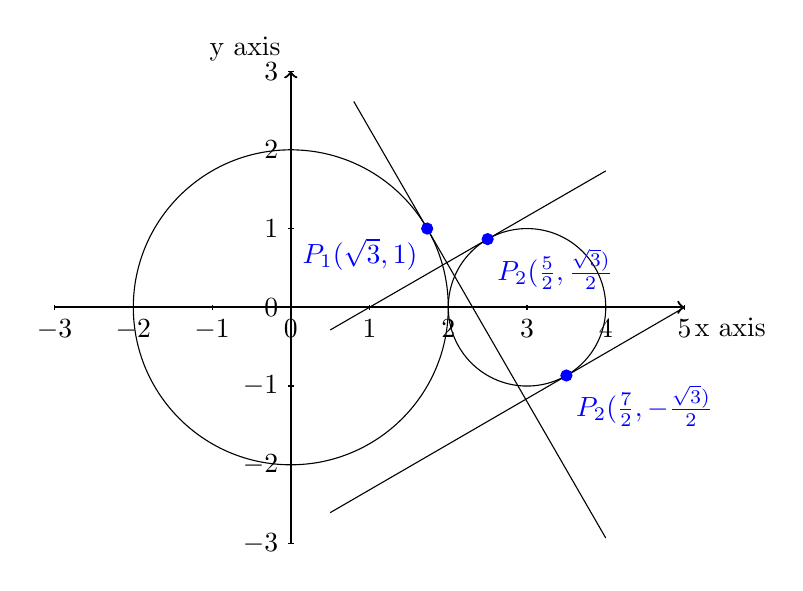
\begin{tikzpicture}
\begin{scope}
\draw[thick,->] (-3,0) -- (5,0) node[anchor=north west] {x axis};
\draw[thick,->] (0,-3) -- (0,3) node[anchor=south east] {y axis};
\foreach \x in {-3,-2,-1,0,1,2,3,4,5}
   \draw (\x cm,1pt) -- (\x cm,-1pt) node[anchor=north] {$\x$};
\foreach \y in {-3,-2,-1,0,1,2,3}
    \draw (1pt,\y cm) -- (-1pt,\y cm) node[anchor=east] {$\y$};
\draw (0,0) circle (2cm);
\draw (3,0) circle (1cm);
\draw (5,0) -- (0.5,-2.608);
\draw (0.5,-0.288) -- (4,1.732);
\draw (0.8,2.614) -- (4,-2.93);
\filldraw[blue](1.732,1) circle (2pt) node[anchor=north east] {$P_{1}(\sqrt{3},1)$};
\filldraw[blue](3.5,-0.866) circle (2pt) node[anchor=north west] {$P_{2}(\frac{7}{2},-\frac{\sqrt{3})}{2}$};
\filldraw[blue](2.5,0.866) circle (2pt) node[anchor=north west] {$P_{2}(\frac{5}{2},\frac{\sqrt{3})}{2}$};
\end{scope}
\end{tikzpicture}
\end{frame}


%----------------------------------------------------------------------------------------

\end{document}